% A tagged Riemann sum: rectangles over a partition of [a,b] with sample
% points xi_i, the rectangle heights being f(xi_i).
% Source: book/tex/calculus/integrate.tex (§ The Riemann integral).
\documentclass[border=2mm]{standalone}
\usepackage{tikz}
\begin{document}
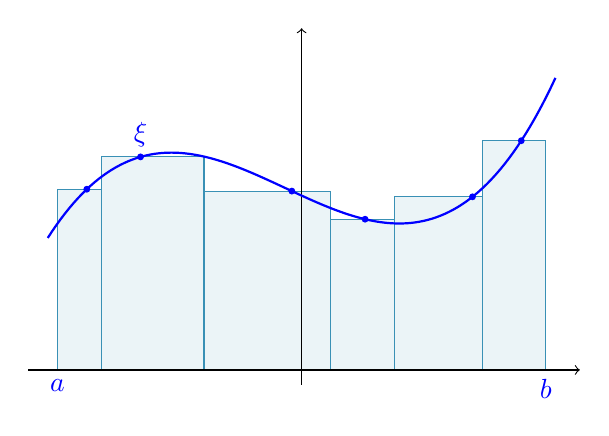
\begin{tikzpicture}[scale=0.62]
  \foreach \lx/\rx/\s in {-5/-4.1/-4.4, -4.1/-2/-3.3, -2/0.6/-0.2,
                          0.6/1.9/1.3, 1.9/3.7/3.5, 3.7/5/4.5} {
    \pgfmathsetmacro\h{3+(\s-2)*(\s-2)*(\s+5)/35}
    \fill[cyan!70!black,opacity=0.1] (\lx,0) rectangle (\rx,\h);
    \draw[cyan!70!black] (\lx,0) rectangle (\rx,\h);
    \fill[blue] (\s,\h) circle (2pt);
  }
  \draw[->] (-5.6,0)--(5.7,0);
  \draw[->] (0,-0.3)--(0,7);
  \draw[blue,thick,domain=-5.2:5.2,samples=120]
    plot (\x, {3+(\x-2)*(\x-2)*(\x+5)/35});
  \node[blue,above] at (-3.3,{3+(-3.3-2)*(-3.3-2)*(-3.3+5)/35}) {$\xi$};
  \node[blue,below] at (-5,0) {$a$};
  \node[blue,below] at (5,0) {$b$};
\end{tikzpicture}
\end{document}
